\let\negmedspace\undefined
\let\negthickspace\undefined
\documentclass[journal]{IEEEtran}
\usepackage[a4paper, margin=10mm, onecolumn]{geometry}
\usepackage{lmodern} % Ensure lmodern is loaded for pdflatex
\usepackage{tfrupee} % Include tfrupee package

\setlength{\headheight}{1cm} % Set the height of the header box
\setlength{\headsep}{0mm}  % Set the distance between the header box and the top of the text

\usepackage{gvv-book}
\usepackage{gvv}
\usepackage{cite}
\usepackage{amsmath,amssymb,amsfonts,amsthm}
\usepackage{algorithmic}
\usepackage{graphicx}
\usepackage{float}
\usepackage{textcomp}
\usepackage{xcolor}
\usepackage{txfonts}
\usepackage{listings}
\usepackage{enumitem}
\usepackage{mathtools}
\usepackage{gensymb}
\usepackage{comment}
\usepackage[breaklinks=true]{hyperref}
\usepackage{tkz-euclide} 
\usepackage{listings}
% \usepackage{gvv}                                        
\def\inputGnumericTable{}                                 
\usepackage[latin1]{inputenc}                                
\usepackage{color}                                            
\usepackage{array}                                            
\usepackage{longtable}                                       
\usepackage{calc}                                             
\usepackage{multirow}                                         
\usepackage{hhline}                                           
\usepackage{ifthen}                                           
\usepackage{lscape}
\usepackage{tikz}
\usetikzlibrary{patterns}

\begin{document}

\bibliographystyle{IEEEtran}
\vspace{3cm}

\title{9.8.1}
\author{EE25BTECH11064 - Yojit Manral}

\maketitle
% \maketitle
% \newpage
% \bigskip
{\let\newpage\relax\maketitle}
\renewcommand{\thefigure}{\theenumi}
\renewcommand{\thetable}{\theenumi}
\setlength{\intextsep}{10pt} % Space between text and float

\textbf{Question:}\\
The line $x + 3y = 0$ is the diameter of the circle $x^2 + y^2 - 6x + 2y = 0$.

\textbf{Solution:}\\
$\rightarrow$ The given circle can be expressed as
\begin{align}
    \vec{x}^T\vec{V}\vec{x} + 2\vec{u}^T\vec{x} + f = 0 \\
    \vec{V} = \myvec{1&0\\0&1}\text{, } \vec{u} = \myvec{-3\\1}\text{, } f = 0
\end{align}
$\rightarrow$ Also, the center of the circle is
\begin{align}
    \vec{c} &= -\vec{V}^{-1}\vec{u}\text{; } |\vec{V}| \neq 0 \\
    \vec{c} &= \myvec{3\\-1}
\end{align}
$\rightarrow$ The given line can be expressed as
\begin{align}
    \vec{x} = \vec{h} + \kappa\vec{m}\text{; } \kappa \in R\\
    \vec{h} = \myvec{0\\0}\text{, } \vec{m} = \myvec{3\\-1}
\end{align}
$\rightarrow$ If the line is a diameter of the circle, the center of the circle must lie on the line
\begin{align}
    \vec{c} &= \vec{h} + \lambda \vec{m} \hspace{0.2cm} \exists \hspace{0.1cm} \lambda \in R \\
    \myvec{3\\-1} &= \myvec{0\\0} + \lambda \myvec{3\\-1} \\
    \lambda &= 1 \in R
\end{align}
$\implies$ Center of circle, $\vec{c}$ lies on the line
$\implies$ The line is a diameter of the circle
\begin{figure}[h!]
   \centering
   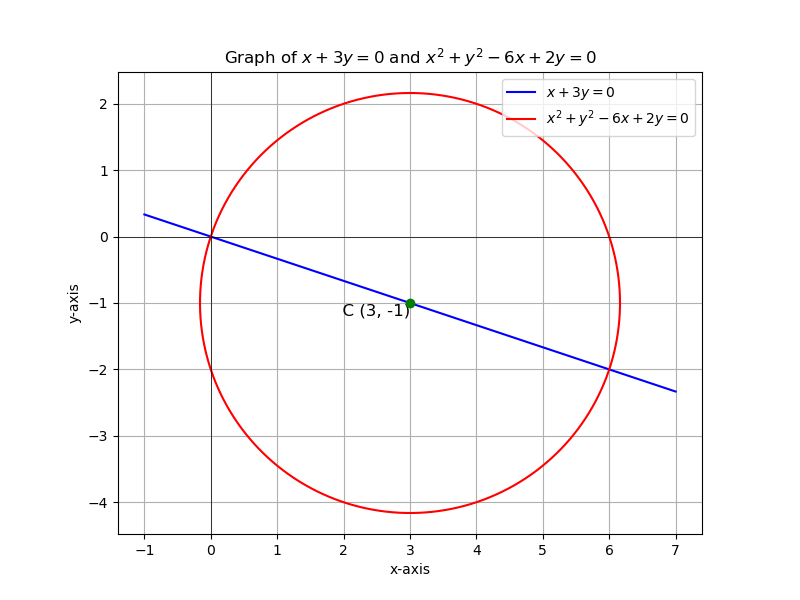
\includegraphics[width=0.8\linewidth]{figs/01.png}
   \caption{Plot of given line and circle}
   \label{Plot_1}
\end{figure}
\end{document}
